\documentclass{beamer}
\usepackage[utf8]{inputenc}
\usepackage[brazil]{babel}
\usepackage{pgfplots}
\usepackage{tikz}
\usepackage{amssymb}
\usepackage{mathtools}

\usetheme{Madrid}
\usecolortheme{default}


\title{Amostragem de Sinal Contínuo}

\author{\textbf{Pierre Machado} \and \textbf{Pedro Fernandes}}

\institute{\textbf{UEFS}}

\date{18 de Setembro de 2026}

\AtBeginSection[]
{
  \begin{frame}
    \frametitle{Sumário}\tableofcontents[currentsection]
  \end{frame}
}


\begin{document}

%The next statement creates the title page.
\frame{\titlepage}


%---------------------------------------------------------
%This block of code is for the table of contents after
%the title page
\begin{frame}
\frametitle{Sumário}
\tableofcontents
\end{frame}
%---------------------------------------------------------


\section{Introdução}
\subsection{Problema Proposto;}

\begin{frame}{Problema Proposto}

\begin{columns}

    \column{0.5\textwidth}

    \begin{itemize}
    \item Avaliar o teorema da amostragem de sinais contínuos no tempo;
    \item Analisar analiticamente os métodos de amostragem ideal, natural e flat-top;
    \item Comparar as características dos métodos.
\end{itemize}

    \column{0.5\textwidth}

    \begin{figure}
        \centering
        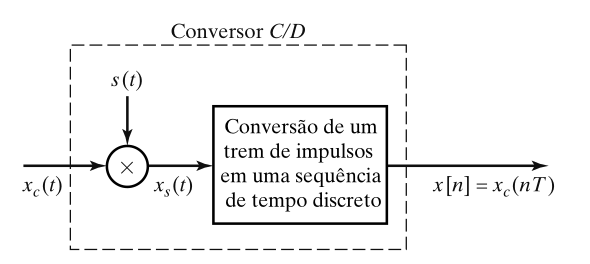
\includegraphics[width=\linewidth]{Imagens/1.png}
        \caption{Sistema total de amostragem. Fonte: Adaptado de: (Oppenheim, 2013).}
        \label{fig1}
    \end{figure}
\end{columns}

\end{frame}

\subsection{Filtragem do Sinal;}

\begin{frame}{Filtragem do sinal}

\begin{columns}
    \column{0.5\textwidth}

    \begin{itemize}
        \item No mundo real, um sinal medido geralmente contém
              componentes em várias frequências;
        \item Atenuar frequências indesejáveis e preservar a faixa
              espectral de interesse;
        \item Limitar o sinal a uma determinada banda de frequências
              por meio de frequências de corte;
        \item Modular o sinal para obter a banda de interesse.
    \end{itemize}

    \column{0.5\textwidth}

    \begin{figure}
    \centering
    \hspace*{0.08\textwidth}
    \begin{tikzpicture}
        \begin{axis}[
            width=0.85\textwidth,
            height=0.55\textwidth,
            xlabel={$\omega$},
            ylabel={$H(j\omega)$},
            xmin=-3, xmax=3,
            ymin=-0.1, ymax=1.2,
            xtick={-2,0,2},
            xticklabels={$-\omega_c$, $0$, $\omega_c$},
            ytick=\empty,
            grid=none,
            axis lines=middle,
            axis line style={->},
            xlabel style={below right},
            ylabel style={
                at={(axis description cs:0.53,1.0)},
                anchor=west
            },
        ]

        % Pulso
        \addplot[
            thick,
            const plot
        ] coordinates {
            (-3,0)
            (-2,0)
            (-2,1)
            (2,1)
            (2,0)
            (3,0)
        };

        \end{axis}
    \end{tikzpicture}

    \caption{Representação do espectro do filtro. Fonte: Elaboração própria.}
    \label{fig2}
\end{figure}

\end{columns}
    
\end{frame}

\subsection{Teorema da Amostragem;}

\begin{frame}{Teorema da Amostragem}
    \textbf{Teorema da amostragem de Nyquist-Shannon:} Seja $x(t)$ um sinal de banda limitada com
    
    \begin{equation}
        X(f) = 0 \qquad \text{para} \qquad |f| \geq f_N
    \end{equation}
    
    Então, $x(t)$ é determinado unicamente por suas amostras $x[n] = x(nT_s)$, $n = 0, ±1, ±2, ...$, se
    
    \begin{equation}
        f_s = \frac{2\pi}{T_s} > 2 \cdot f_N
    \end{equation}

    Em que:
    \begin{itemize}
        \item $f_N$ é a frequência máxima do sinal;
        \item $f_s$ é a frequência de amostragem;
        \item $T_s$ é o período de amostragem.
    \end{itemize}
\end{frame}

\subsection{Aliasing e Critério de Nyquist}

\begin{frame}{Critério de Nyquist e Aliasing}

        \begin{columns}

            \column{0.5\textwidth}

            \begin{itemize}
                \item O critério de Nyquist, derivado do Teorema da Amostragem, afirma que um sinal pode ser reconstruído a partir de suas amostras desde que a $f_s > 2f_N$.
            \end{itemize}

            \begin{figure}
                \centering
                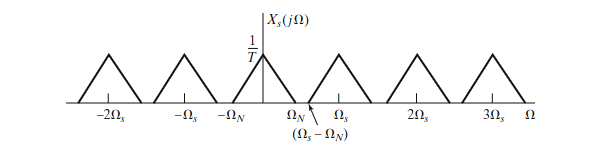
\includegraphics[width=1.1\linewidth]{Imagens/2.png}
                \caption{Réplicas Espectrais do Sinal Amostrado sem \textit{aliasing}. Fonte: (Oppenheim, 2013)}
                \label{fig2}
            \end{figure}

            \column{0.5\textwidth}
    
            \begin{itemize}
                \item Quando o critério de Nyquist não é atendido, as réplicas espectrais do sinal amostrado se sobrepõem, produzindo o fenômeno de \textit{aliasing}.
            \end{itemize}
    
            \begin{figure}
                \centering
                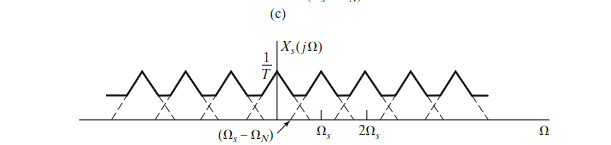
\includegraphics[width=1.1\linewidth]{Imagens/3.png}
                \caption{Réplicas Espectrais do Sinal Amostrado com \textit{aliasing}. Fonte: (Oppenheim, 2013)}
                \label{fig3}
            \end{figure}
            
        \end{columns}


\end{frame}

\section{Desenvolvimento}

\subsection{Amostragem Ideal}

    \begin{frame}{Amostragem ideal}
        \begin{columns}

            \column{0.5\linewidth}

            \begin{itemize}
                \item Amostragem ideal é o método matemático em que um sinal contínuo $x(t)$ é convertido em uma sequência de valores instantâneos tomados em intervalos regulares de tempo.
                \item Se o período de amostragem é $T_s$, então $x[n] = x(nT_s)\textit{,} \quad \text{para} \quad n \in \mathbb{Z}$
            \end{itemize}

            \column{0.5\linewidth}

            \begin{figure}
            \centering
            
            \begin{tikzpicture}
            \begin{axis}[
                width=0.85\textwidth,
                height=5.5cm,
                xmin=0, xmax=2*pi,
                ymin=-1.3, ymax=1.3,
                domain=0:2*pi,
                samples=500,
                axis lines=middle,
                axis line style={->},
                xlabel={$t$},
                ylabel={$x(t)$},
                xtick=\empty,
                ytick=\empty,
                grid=none,
                xlabel style={below right},
                ylabel style={above left},
            ]
            
            % Sinal contínuo
            \addplot[
                thick
            ]
            {sin(deg(x))};
            
            % Retas verticais de amostragem
            \foreach \x in {0,pi/4,pi/2,3*pi/4,pi,5*pi/4,3*pi/2,7*pi/4,2*pi}{
                \addplot[
                    thick
                ]
                coordinates {
                    (\x,0)
                    (\x,{sin(deg(\x)})
                };
            }
            
            % Marcação dos valores x(nTs)
            \addplot[
                only marks,
                mark=*,
                mark size=1.5pt,
                color=blue
            ]
            coordinates {
                (0,0)
                (pi/4,0.7071)
                (pi/2,1)
                (3*pi/4,0.7071)
                (pi,0)
                (5*pi/4,-0.7071)
                (3*pi/2,-1)
                (7*pi/4,-0.7071)
                (2*pi,0)
            };

            % Indicação do período de amostragem Ts
            \draw[<->, thick]
                (axis cs:0,-0.15) --
                node[below] {$T_s$}
                (axis cs:pi/4,-0.15);
            
            \end{axis}
            \end{tikzpicture}
            
            \caption{Representação da amostragem ideal de um sinal senoidal. Fonte: Elaboração Própria}
            
            \end{figure}
        
        \end{columns}
\end{frame}

\begin{frame}{Avaliação Analítica no Domínio do Tempo}
    Seja $s(t)$ um trem periódico de impulsos, com impulsos espaçados por um período $T_s$, e $x(t)$ o sinal a ser amostrado.

    \begin{equation}
        s(t) = \displaystyle\sum_{k = -\infty}^{+\infty}\delta(t-kT_s)
    \end{equation}

    $s(t)$ pode ser representado em termos da Série de Fourier, por ser um sinal periódico (Oppenheim, 2010).

    \begin{equation}
        s(t) = \frac{1}{T_s} \displaystyle\sum_{k = -\infty}^{+\infty}e^{jk2\pi f_st}
    \end{equation}

\end{frame}

\begin{frame}{Avaliação Analítica no Domínio da Frequência}
    Multiplicam-se os sinais para obter amostras do sinal $x(t)$ nos instantes correspondentes a múltiplos inteiros do período de amostragem $T_s$. Dessa forma, obtém-se a amostragem ideal do sinal.

    \begin{equation}
        x_s(t) = x(t) \cdot s(t) = \frac{1}{T_s}\displaystyle\sum_{k = -\infty}^{+\infty}x(t)e^{jk2\pi f_st}
    \end{equation}

Pela propriedade de homogeneidade e deslocamento no tempo da transformada de Fourier(Oppenheim, 2010)\footnote{$
a\,x(t) \leftrightarrow a\,X(f), \quad x(t)e^{j2\pi f_0t} \leftrightarrow X(f-f_0)$}, obtém-se o espectro do sinal amostrado.

    \begin{equation}
        X_s(f) = \frac{1}{T_s}\displaystyle\sum_{k = -\infty}^{+\infty}X(f-kf_s)
    \end{equation}

\end{frame}

\begin{frame}{Visualização do Espectro da Amostragem Ideal}
    \begin{exampleblock}{Exemplo de Espectro de Amostragem Idealmente}
        Considere o espectro do sinal na Figura à esquerda. O espectro da amostragem ideal são as réplicas do espectro do sinal original, como mostra a Figura à direita, ponderadas pela frequência de amostragem.
    \end{exampleblock}

    \begin{columns}[t]
    
        \column{0.5\linewidth}
    
        \begin{figure}[H]
            \centering
            \begin{tikzpicture}
    
            \def\B{1}
    
            \begin{axis}[
                axis lines=middle,
                xlabel={$f$},
                ylabel={$X(f)$},
                xlabel style={font=\scriptsize},
                ylabel style={font=\scriptsize},
                xticklabel style={font=\scriptsize},
                xmin=-5, xmax=5,
                ymin=0, ymax=1.2,
                xtick={-1,0,1},
                xticklabels={$-f_N$,$0$,$f_N$},
                ytick=\empty,
                width=0.95\linewidth,
                height=0.48\linewidth,
                clip=false
            ]
    
            \addplot[
                thick,
                domain=-1:1,
                samples=50
            ]
            {max(0,1-abs(x)/\B)};
    
            \end{axis}
    
            \end{tikzpicture}
    
            \caption{Espectro do sinal $X(f)$. Fonte: Elaboração própria.}
        \end{figure}
    
        \column{0.5\linewidth}
    
        \begin{figure}[H]
            \centering
            \begin{tikzpicture}
    
            \def\fs{3}
            \def\B{1}
    
            \begin{axis}[
                axis lines=middle,
                xlabel={$f$},
                ylabel={$X_s(f)$},
                xlabel style={font=\scriptsize},
                ylabel style={font=\scriptsize},
                xticklabel style={font=\scriptsize},
                xmin=-5, xmax=5,
                ymin=0, ymax=1.2,
                xtick={-3,0,3},
                xticklabels={$-f_s$,$0$,$f_s$},
                ytick=\empty,
                width=0.95\linewidth,
                height=0.48\linewidth,
                clip=false
            ]
    
            % Réplica em -fs
            \addplot[
                thick,
                domain=-4:-2,
                samples=50
            ]
            {max(0,1-abs(x+3)/\B)};
    
            % Espectro original
            \addplot[
                thick,
                domain=-1:1,
                samples=50
            ]
            {max(0,1-abs(x)/\B)};
    
            % Réplica em fs
            \addplot[
                thick,
                domain=2:4,
                samples=50
            ]
            {max(0,1-abs(x-3)/\B)};
    
            % Pontos à esquerda
            \addplot[
                only marks,
                mark=*,
                mark size=0.7pt
            ] coordinates {
                (-4.5,0.5)
                (-4.7,0.5)
                (-4.9,0.5)
            };
    
            % Pontos à direita
            \addplot[
                only marks,
                mark=*,
                mark size=0.7pt
            ] coordinates {
                (4.5,0.5)
                (4.7,0.5)
                (4.9,0.5)
            };
    
            % Linhas indicando os múltiplos de fs
            \draw[dashed] (axis cs:-3,0) -- (axis cs:-3,1);
            \draw[dashed] (axis cs:3,0) -- (axis cs:3,1);
    
            \end{axis}
    
            \end{tikzpicture}
    
            \caption{Réplicas espectrais do sinal amostrado, espaçadas por múltiplos da frequência de amostragem $f_s$. Fonte: Elaboração própria.}
        \end{figure}
    
    \end{columns}
\end{frame}

% \displaystyle\sum_{n = -\infty}^{+\infty}\delta(t-nT_s)$

\subsection{Amostragem Natural}

\begin{frame}{Amostragem Natural}
    \begin{columns}
        \column{0.5\linewidth}
    
        \begin{itemize}
            \item A amostragem natural é um método em que um sinal contínuo \(x(t)\) é multiplicado por um trem periódico de pulsos retangulares de largura finita \(\tau\), espaçados regularmente pelo período de amostragem \(T_s\); 
            \item Durante cada pulso, o sinal amostrado acompanha a forma do sinal original, resultando em segmentos de \(x(t)\) que são periodicamente selecionados ao longo do tempo.
        \end{itemize}

        \column{0.5\linewidth}

        \begin{figure}
            \centering
            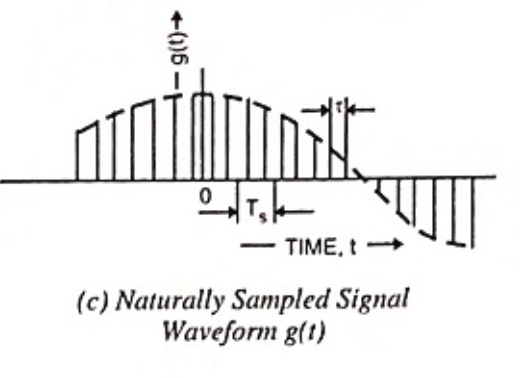
\includegraphics[width=0.75\linewidth]{Imagens/4.png}
            \caption{Amostragem Natural. Fonte: EEEGUIDE.COM, ``Types of Sampling Techniques''.}
        \end{figure}
    \end{columns}
\end{frame}

\begin{frame}{Avaliação Analítica no Domínio do Tempo}
    Seja $x(t)$ o sinal contínuo a ser amostrado e $p(t)$ um trem periódico de pulsos retangulares, com largura $\tau$ e período de amostragem $T_s$.
    \begin{equation}
        p(t) = \displaystyle\sum_{n = -\infty}^{+\infty}p_0(t-nT_s)
    \end{equation}

    \begin{equation}
        p_0(t)= \begin{cases}
        1, & |t|<\dfrac{\tau}{2},\\[7pt]
        0, & |t|\geq\dfrac{\tau}{2}.
        \end{cases}
    \end{equation}

    Devido à periodicidade do trem de pulsos $p(t)$, este pode ser representado por meio de sua Série de Fourier em Tempo Contínuo.

    \begin{equation}
        p(t)=\sum_{k=-\infty}^{+\infty} C_k \cdot e^{j2\pi kf_s t}
    \end{equation}
\end{frame}

\begin{frame}{Coeficientes de Fourier}
    Como $p(t)$ é um sinal periódico, é possível calcular os coeficientes da representação para sinais periódicos da Série de Fourier (Oppenheim, 2010)\footnote{$a_n=\frac{1}{T}\int_{<T>}p(t)e^{-j2\pi nf t}\,dt$}.

    \begin{equation}
        C_k=\frac{1}{T_s}\int_{-\frac{\tau}{2}}^{\frac{\tau}{2}}e^{-j2\pi nf t}dt
    \end{equation}

    \begin{equation}
        C_k=\frac{1}{T_s}
        \left[
        \frac{1}{-j2\pi kf_s}e^{-j2\pi kf_s t}
        \right]_{-\tau/2}^{\tau/2} = \frac{1}{T_s}\frac{\sin(\pi kf_s\tau)}{\pi kf_s}
    \end{equation}

    \begin{equation}
        C_k = \frac{\tau}{T_s}\operatorname{sinc}\left(k\frac{\tau}{T_s}\right)
    \end{equation}
\end{frame}

\begin{frame}{A transformada de Fourier e Modulação no tempo}
    Aplica-se $C_k$ na definição da série de Fourier, após se aplica a transformada de Fourier para obter $P(f)$. A modulação de $p(t)$ com $x(t)$ no tempo, como dito anteriormente, corresponde à convolução no domínio da frequência para obter o espectro do sinal amostrado $X_s(f)$. 

    \begin{equation}
        p(t)=\frac{\tau}{T_s}\sum_{k=-\infty}^{\infty}\operatorname{sinc}\left(k\frac{\tau}{T_s}\right)e^{j2\pi kf_s t}
    \end{equation}

    Obtém-se, pelas propriedades de linearidade e de deslocamento no domínio da frequência, a relação:

    \begin{equation}
        P(f)=\frac{\tau}{T_s}\sum_{k=-\infty}^{\infty}\operatorname{sinc}\left(k\frac{\tau}{T_s}\right)\delta(f-kf_s)
    \end{equation}

    Analisa-se, portanto, a convolução no domínio da frquência:

    \begin{equation}
        X_s(f) = X(t) * P(f)
    \end{equation}
        
\end{frame}

\begin{frame}{Avaliação Analítica no Domínio da Frequência}
    Pela propriedade de convolução com trem de pulsos (Oppenheim, 2010)\footnote{$X(f)*\delta(f-kf_s)=X(f-kf_s)$}, é possível obter o espectro da frequência da amostragem natural.

    \begin{equation}
        X_s(f)=\frac{\tau}{T_s}\sum_{k=-\infty}^{\infty}\operatorname{sinc}\left(k\frac{\tau}{T_s}\right)X(f-kf_s)
    \end{equation}

    Nota-se, portanto, que, assim como na amostragem ideal, há réplicas espectrais no domínio da frequência do sinal amostrado. Porém, a diferença está na ponderação das réplicas.
\end{frame}

\begin{frame}{Visualização do Espectro da Amostragem Natural}

\begin{exampleblock}{Exemplo de Espectro de Amostragem Natural}
    O espectro da amostragem natural mostra as réplicas do espectro do sinal original, como mostra a Figura, ponderadas pelo fator $\frac{\tau}{T_s} \cdot \operatorname{sinc}\left(k\frac{\tau}{T_s}\right)$
\end{exampleblock}

\begin{figure}[H]
    \centering
    \begin{tikzpicture}

    \begin{axis}[
        axis lines=middle,
        xlabel={$f$},
        ylabel={$X_s(f)$},
        xlabel style={font=\tiny, below=1.5pt},
        ylabel style={font=\tiny},
        xtick={-5,-2.5,0,2.5,5},
        xticklabels={$-2f_s$,$-f_s$,$0$,$f_s$,$2f_s$},
        ytick=\empty,
        xticklabel style={font=\tiny},
        xmin=-7,
        xmax=7,
        ymin=0,
        ymax=1.15,
        width=1.00\linewidth,
        height=0.50\linewidth,
        clip=false
    ]

    % Parâmetros
    \def\fs{2.5}
    \def\B{1}

    % =========================================
    % RÉPLICA k = -2
    % =========================================

    \addplot[
        thick,
        domain=-6:-4,
        samples=50
    ]
    {
        0.20*max(0,1-abs(x+5)/\B)
    };


    % =========================================
    % RÉPLICA k = -1
    % =========================================

    \addplot[
        thick,
        domain=-3.5:-1.5,
        samples=50
    ]
    {
        0.60*max(0,1-abs(x+2.5)/\B)
    };


    % =========================================
    % RÉPLICA CENTRAL k = 0
    % =========================================

    \addplot[
        thick,
        domain=-1:1,
        samples=50
    ]
    {
        1.00*max(0,1-abs(x)/\B)
    };


    % =========================================
    % RÉPLICA k = +1
    % =========================================

    \addplot[
        thick,
        domain=1.5:3.5,
        samples=50
    ]
    {
        0.60*max(0,1-abs(x-2.5)/\B)
    };


    % =========================================
    % RÉPLICA k = +2
    % =========================================

    \addplot[
        thick,
        domain=4:6,
        samples=50
    ]
    {
        0.20*max(0,1-abs(x-5)/\B)
    };


    % =========================================
    % LINHAS VERTICAIS EM k f_s
    % =========================================

    \foreach \x/\h in {
        -5/0.20,
        -2.5/0.60,
         0/1.00,
         2.5/0.60,
         5/0.20
    }{
        \addplot[
            thin,
            dashed
        ]
        coordinates {
            (\x,0)
            (\x,\h)
        };
    }

    \node[font=\Large] at (axis cs:-6.5,0.575) {$\cdots$};
    \node[font=\Large] at (axis cs:6.5,0.575) {$\cdots$};
    
    \end{axis}

    \end{tikzpicture}

    \caption{Espectro da Amostragem Natural. Fonte: Elaboração própria.}

\end{figure}
\end{frame}

\subsection{Amostragem Flat-Top}

\begin{frame}{Amostragem Flat-Top}

    \begin{columns}
        \column{0.5\linewidth}

        \begin{itemize}
            \item A amostragem Flat-Top é um método de amostragem no qual cada amostra do sinal é mantida constante durante um intervalo de duração finita, formando pulsos retangulares de amplitude igual ao valor do sinal no instante de amostragem;
            \item O valor da amostra é mantido constante, produzindo o formato de topo plano.
        \end{itemize}

        \column{0.5\linewidth}

        \begin{figure}
            \centering
            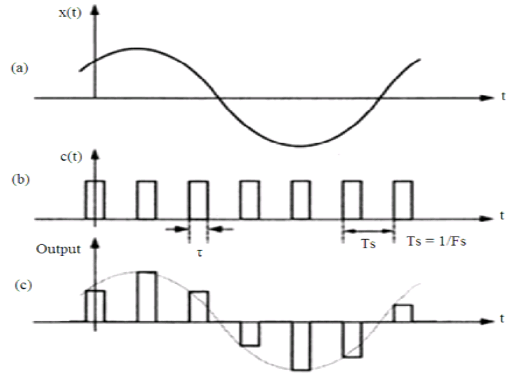
\includegraphics[width=0.75\linewidth]{Imagens/5.png}
            \caption{Amostragem Flat-Top. Fonte: QUES10. "State Sampling theorem. Explain Flat-top sampling. Draw its spectrum and explain Aperture effect."}
        \end{figure}
    \end{columns}
\end{frame}

\begin{frame}{Avaliação Analítica no Domínio do Tempo}
    Seja $x(t)$ um sinal a ser amostrado. Na amostragem de topo plano, o sinal é inicialmente amostrado em instantes $nT_s$ e, em seguida, cada amostra é convoluída com um pulso retangular de largura $\tau$.

    Dessa maneira, é possível definir o sinal amostrado da seguinte maneira

    \begin{equation}
        x_{FT}(t)=[x(t) \cdot \displaystyle\sum_{n=-\infty}^{\infty}\delta(t-nT_s)]*p_0(t)
    \end{equation}

    Com $p_0(t)$ definido logo abaixo:
    
    \begin{equation}
        p_0(t)=\begin{cases}
        1, & |t|<\dfrac{\tau}{2}\\0, & \text{caso contrário}.
        \end{cases}
    \end{equation}
\end{frame}

\begin{frame}{Avaliação Analítica no Domínio da Frequência}

O primeiro fator da convolução, no domínio da frequência, pode ser obtida pela propriedade de convolução com espectro do trem de impulsos (Oppenheim, 2010), já mencionada.

\begin{equation}
    X_{\delta}(f)=f_s\sum_{k=-\infty}^{\infty}X(f-kf_s)
\end{equation}

Considera-se a propriedade de multiplicação no domínio da frequência (Oppenheim, 2010).

\begin{equation}
    X_{FT}(f) = X_{\delta}(f)P_0(f)
\end{equation}

Com o espectro do pulso definido pela função $\operatorname{sinc}$ ponderada:

\begin{equation}
   P_0(f)=\tau\ \cdot \operatorname{sinc}(f\tau)
\end{equation}
    
\end{frame}

\begin{frame}{Avaliação Analítica no Domínio da Frequência}
    Avaliando o produto no domínio da frequência, é possível obter o espectro do sinal amostrado com método topo-plano.

    \begin{equation}
        X_{FT}(f) =f_s\tau\,\operatorname{sinc}(f\tau)\sum_{k=-\infty}^{\infty}X(f-kf_s)
    \end{equation}

    A Figura abaixo mostra o espectro da amostragem de Topo Plano. Observa-se o efeito de abertura, que ocorre devido à duração de cada amostra, causando uma atenuação das componentes de alta frequência.
    
    \begin{figure}
        \centering
        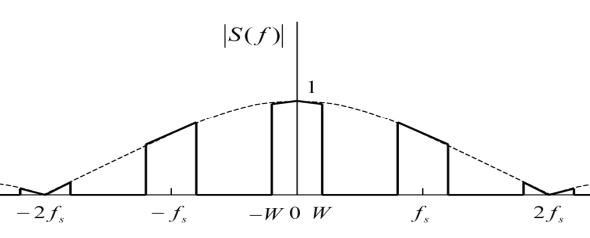
\includegraphics[width=0.5\linewidth]{Imagens/6.png}
        \caption{Fonte: BHARATH INSTITUTE OF HIGHER EDUCATION AND RESEARCH.\textit{Communication Engineering II — BEC604}}
    \end{figure}
\end{frame}

\subsection{Reconstrução do Sinal}

\begin{frame}{Avaliação Analítica da Reconstrução do Sinal}
    \begin{itemize}
        \item A reconstrução do sinal a partir do seu método de amostragem se dá pela Transformada Inversa de Fourier, dada por
            \begin{equation}
                x(t) = \int_{-\infty}^{\infty} X(f) \cdot e^{j2\pi ft} df.
            \end{equation}
        \item Contudo, para cada método de amostragem, também é necessário a realização de ajustes para que o sinal seja reproduzido fielmente, respeitando o critério de Nyquist, no domínio do tempo.
    \end{itemize}
\end{frame}

\begin{frame}{Reconstrução do Sinal por Amostragem Ideal}
    \begin{itemize}
        \item Seja $X_{ideal}(f) = {{1}\over {T_s}} \sum_{k=-\infty}^{\infty}X(f-kfs)$, a reconstrução a partir da amostragem ideal se dá por:
            \begin{itemize}
                \item Isolar a primeira réplica com um filtro passa-baixas, escolhendo uma frequência de corte $f_c$ tal que apenas a réplica em $k=0$ seja mantida (por exemplo, $f_c = f_s/2$);
                \item Aplicar um filtro de ganho, multiplicando a função no domínio da frequência por $T_s$.
            \end{itemize}
    \end{itemize}
\end{frame}

\begin{frame}{Reconstrução do Sinal por Amostragem Ideal}
    \begin{itemize}
        \item Portanto, a reconstrução do sinal no domínio do tempo é:
        \begin{equation}
                    x(t) = {{1}\over {T_s}} \int_{-\infty}^{\infty} \sum_{k=-\infty}^{\infty} X(f-kfs) \cdot e^{j2\pi ft} df
        \end{equation}

        \begin{equation*}
                    x(t) = T_s \cdot {{1}\over {T_s}} \int_{-\infty}^{\infty} X(f-0 \cdot fs) \cdot e^{j2\pi ft} df
        \end{equation*}

        \begin{equation}
                    x(t) = \int_{-\infty}^{\infty} X(f) \cdot e^{j2\pi ft} df.
        \end{equation}

        que é a própria Transformada Inversa de Fourier do sinal $x(t)$ original.
    \end{itemize}
\end{frame}

\begin{frame}{Reconstrução do Sinal por Amostragem Natural}
    \begin{itemize}
        \item De forma semelhante, seja $X_{n}(f) = {{\tau}\over {T_s}} \sum_{k=-\infty}^{\infty} sinc(kf_s \tau) X(f-kfs)$, a reconstrução a partir da amostragem natural se dá por:
            \begin{itemize}
                \item Também isolar a primeira réplica com um filtro passa-baixas, escolhendo uma frequência de corte $f_c$ tal que apenas a réplica em $k=0$ seja mantida;
                \item Aplicar um filtro de ganho, multiplicando a função no domínio da frequência por $\frac{T_s}{\tau}$.
            \end{itemize}
    \end{itemize}
\end{frame}

\begin{frame}{Reconstrução do Sinal por Amostragem Natural}
    \begin{itemize}
        \item Portanto, a reconstrução do sinal no domínio do tempo é:
        \begin{equation}
                    x(t) = {{\tau}\over {T_s}} \int_{-\infty}^{\infty} \sum_{k=-\infty}^{\infty} sinc(kf_s \tau) X(f-kfs) \cdot e^{j2\pi ft} df
        \end{equation}

        \begin{equation*}
                    x(t) = \frac{T_s}{\tau} \cdot {{\tau}\over {T_s}} \int_{-\infty}^{\infty}sinc(0) X(f) \cdot e^{j2\pi ft} df = \int_{-\infty}^{\infty}1 \cdot X(f) \cdot e^{j2\pi ft}
        \end{equation*}

        \begin{equation}
                    x(t) = \int_{-\infty}^{\infty} X(f) \cdot e^{j2\pi ft} df.
        \end{equation}

        que também é a própria Transformada Inversa de Fourier do sinal $x(t)$ original.
    \end{itemize}
\end{frame}

\begin{frame}{Reconstrução do Sinal por Amostragem Topo-Plano}
    \begin{itemize}
        \item Por fim, seja $X_{flat}(f) = {{\tau}\over {T_s}} \cdot sinc(f\tau) \sum_{k=-\infty}^{\infty} X(f-kfs) \cdot e^{-j\pi ft}$, a reconstrução a partir da amostragem topo-plano difere das demais, tendo a sua reconstrução feita da seguinte forma:
            \begin{itemize}
                \item Isolando a primeira réplica com um filtro passa-baixas, escolhendo uma frequência de corte $f_c$ tal que apenas a réplica em $k=0$ seja mantida;
                \item Aplicar um filtro equalizador, multiplicando a função no domínio da frequência por $X_{eq}(f)=\frac{T_s}{\tau} \cdot \frac{1}{sinc(f\tau)} \cdot e^{j\pi ft}$, eliminando assim a componente complexa de defasagem e realizando o ganho da amplitude.
            \end{itemize}
    \end{itemize}
\end{frame}

\begin{frame}{Reconstrução do Sinal por Amostragem Topo-Plano}
    \begin{itemize}
        \item Logo, a reconstrução do sinal no domínio do tempo é:
        \begin{equation}
                    x(t) = {{\tau}\over {T_s}} \cdot sinc(f\tau)\int_{-\infty}^{\infty} \sum_{k=-\infty}^{\infty} X(f-kfs) \cdot e^{-j\pi ft} \cdot e^{j2\pi ft} df
        \end{equation}

        \begin{equation*}
                    x(t) = \frac{T_s}{\tau} \cdot {{\tau}\over {T_s}} \cdot sinc(f\tau) \cdot \frac{1}{sinc(f\tau)} \cdot e^{j\pi ft} \int_{-\infty}^{\infty} X(f) \cdot e^{-j\pi ft} \cdot e^{j2\pi ft} df
        \end{equation*}

        \begin{equation*}
                    x(t) = \int_{-\infty}^{\infty} X(f) \cdot e^{j\pi ft - j\pi ft}\cdot e^{j2\pi ft} df = \int_{-\infty}^{\infty} X(f) \cdot e^{0}\cdot e^{j2\pi ft} df
        \end{equation*}

        \begin{equation}
            x(t) = \int_{-\infty}^{\infty} X(f) \cdot e^{j2\pi ft} df
        \end{equation}

        que, por fim, é a própria Transformada Inversa de Fourier do sinal $x(t)$ original.
    \end{itemize}
\end{frame}

\section{Resultados}

\begin{frame}{Resultados Obtidos}
\begin{itemize}
    \item Foram realizadas simulações computacionais no \textit{GNU Octave}
para a análise dos processos de amostragem, permitindo visualizar
os sinais no domínio do tempo e seus respectivos espectros no
domínio da frequência.
    \item A amostragem ideal fornece um modelo matemático baseado em impulsos
de Dirac. A amostragem natural utiliza pulsos de duração finita,
durante os quais o sinal mantém sua variação original. Na amostragem
de Topo Plano, o valor instantâneo da amostra é mantido constante durante
o intervalo de abertura, introduzindo uma envoltória do tipo
$\operatorname{sinc}(f\tau)$ no espectro, associada ao efeito de
abertura.
\end{itemize}

\end{frame}

\begin{frame}{Referências}
    \footnotesize

    \begin{thebibliography}{99}

    \bibitem{oppenheim-sinais}
    OPPENHEIM, Alan V.; WILLSKY, Alan S.; NAWAB, S. Hamid.
    \textit{Sinais e sistemas}.
    2. ed. São Paulo: Pearson Prentice Hall, 2010.

    \bibitem{oppenheim-processamento}
    OPPENHEIM, Alan V.; SCHAFER, Ronald W.; BUCK, John R.
    \textit{Processamento em tempo discreto de sinais}.
    2. ed. São Paulo: Pearson Prentice Hall, 2009.

    \bibitem{eeeguide}
    EEEGUIDE.COM.
    \textit{Types of Sampling Techniques}.
    Disponível em:
    \url{https://www.eeeguide.com/types-of-sampling-techniques/}.
    Acesso em: 17 set. 2026.

    \bibitem{ques10}
    QUES10.
    \textit{State Sampling theorem. Explain Flat-top sampling.
    Draw its spectrum and explain Aperture effect}.
    Disponível em:
    \url{https://www.ques10.com/p/11457/state-sampling-theorem-explain-flat-top-sampling-d/}.
    Acesso em: 17 set. 2026.

    \bibitem{bharath}
    BHARATH INSTITUTE OF HIGHER EDUCATION AND RESEARCH.
    \textit{Communication Engineering II -- BEC604}.
    Disponível em:
    \url{https://www.bharathuniv.ac.in/colleges1/downloads/courseware_ece/notes/BEC604\%20-COMMUNICATION\%20ENG\%20II.pdf}.
    Acesso em: 17 set. 2026.

    \end{thebibliography}
\end{frame}


\end{document}